\subsection{Structure of \texorpdfstring{$\E[\vx\vx^\T]$}{ExxT} and \texorpdfstring{$\E[\mM]$}{EM} During Training}
\label{sec:appendix_training_traj}
We observed the pattern of $\E[\vx\vx^\T]$ matrix and $\E[\mM]$ matrix along the training trajectory (\figureref{fig:traj_xxT_lenet5_fc1}, \figureref{fig:traj_UTAU_lenet5_fc1}). It shows that $\E[\vx\vx^\T]$ is always approximately rank 1, and $\E[\mM]$ always have around $c$ large eigenvalues. According to our analysis, since the nontrivial eigenspace overlap is likely to be a consequence of a approximately rank 1 $\E[\vx\vx^\T]$, we would conjecture that the overlap phenomenon is likely to happen on the training trajectory as well.

\begin{figure}[H]
    \centering
    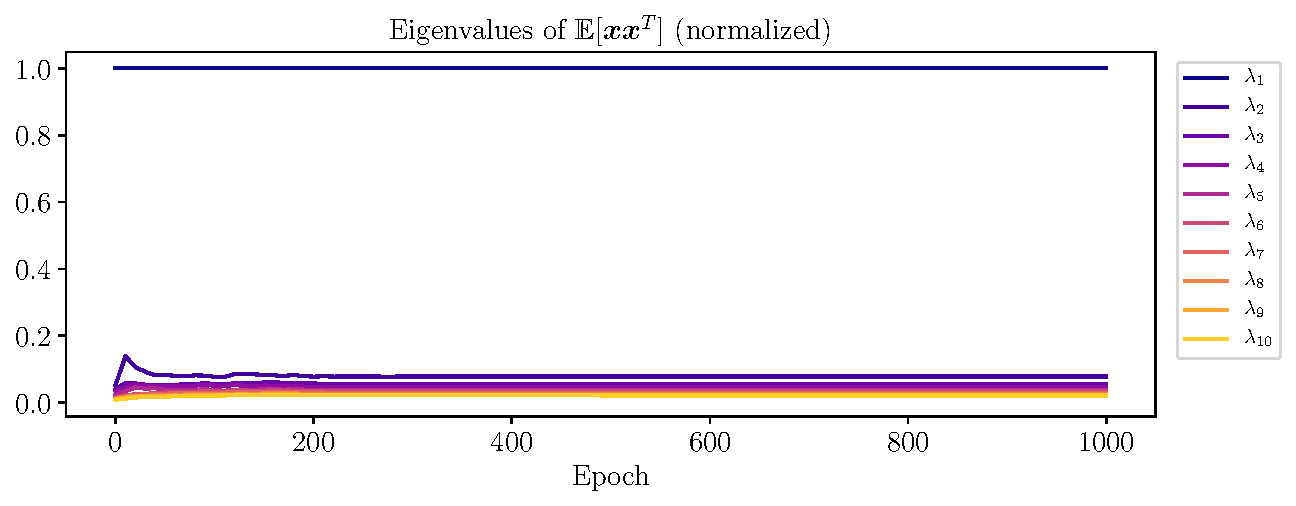
\includegraphics[height=0.2\textheight]{Appendix_Figures/Along_traj/ExxT_val/ExxT_trend_10_CIFAR10_Exp1_LeNet5_fixlr0.01R1_0_1000_fc1.pdf}
    % \captionsetup{justification=centering}
    \caption{Top eigenvalues of $\E[\vx\vx^\T]$ along training trajectory. (fc1:LeNet5)}
    \label{fig:traj_xxT_lenet5_fc1}
\end{figure}

\begin{figure}[H]
    \centering
    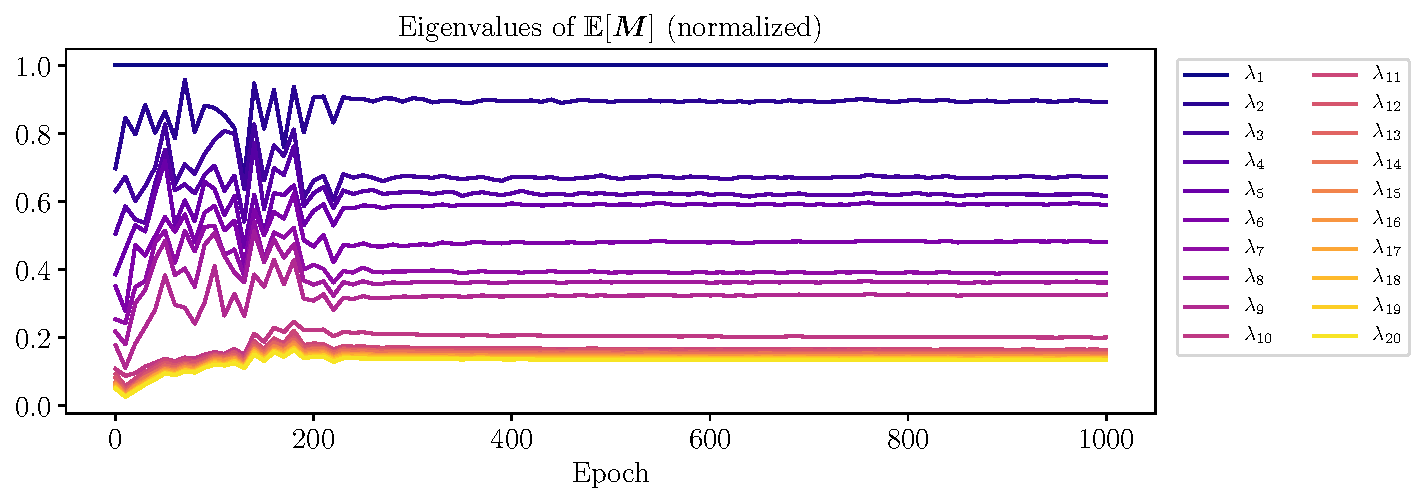
\includegraphics[height=0.2\textheight]{Appendix_Figures/Along_traj/UTAU_val/EUTAU_trend_20_CIFAR10_Exp1_LeNet5_fixlr0.01R1_0_1000_fc1.pdf}
    % \captionsetup{justification=centering}
    \caption{Top eigenvalues of $\E[\mM]$ along training trajectory. (fc1:LeNet5)}
    \label{fig:traj_UTAU_lenet5_fc1}
\end{figure}